\documentclass[11pt]{article}
\usepackage[T1]{fontenc}
\usepackage[utf8]{inputenc}
\usepackage{listings}
\usepackage{xcolor}
\usepackage{graphicx}
\definecolor{codegreen}{rgb}{0,0.6,0}
\definecolor{codegray}{rgb}{0.5,0.5,0.5}
\definecolor{codepurple}{rgb}{0.58,0,0.82}
\definecolor{backcolour}{rgb}{0.95,0.95,0.92}

\lstdefinestyle{mystyle}{
    backgroundcolor=\color{backcolour},   
    commentstyle=\color{codegreen},
    keywordstyle=\color{magenta},
    numberstyle=\tiny\color{codegray},
    stringstyle=\color{codepurple},
    basicstyle=\ttfamily\footnotesize,
    breakatwhitespace=false,         
    breaklines=true,                 
    captionpos=b,                    
    keepspaces=true,                 
    numbers=left,                    
    numbersep=5pt,                  
    showspaces=false,                
    showstringspaces=false,
    showtabs=false,                  
    tabsize=2
}

\lstset{style=mystyle}
\title{Algorytm genetyczny dla \\ problemu komiwojażera}
\author{Piotr Popis}
\date{Czerwiec 2020}
\begin{document}
\begin{titlepage}
\maketitle
\end{titlepage}
\section{Wprowadzenie}
\subsection{Problem komiwojażera( Traveling Salesman Problem)}
Jest jednym z najszerzej przebadanych problemów optymalizacji kombinatorycznej. Polega na zminimalizowaniu dystansu trasy Salesmana, gdzie trasa musi przechodzić przez zadane $n$ ( załóżmy, że ) $miast$ z jego listy, które powinien przejść dokładanie raz oraz znane są odległości pomiędzy miastami. Inaczej mówiąc szukamy minimalnego cyklu Hamiltona w pełnym grafie ważonym.\\
Problem możemy przedstawiać w różnych wariantach na przykład:
\begin{enumerate}
\item symetryczny sTSP
\item asymetryczny aTSP
\item wielokrotny mTSP
\item zgeneralizowany gTSP
\end{enumerate}
W symetrycznym przypadku odległość z miasta A do B jest taka sama jak odległość z B do A. W asymetrycznym odległości te mogą być różne ( $c_{ij} \neq c_{ji}$). W 3 przypadku wielokrotnym miasto może być odwiedzone więcej niż raz, a w przypadku zgeneralizowanym( uogólnionym) nie wszystkie miasta muszą być odwiedzone.
   Tego typu problemy powstają w różnych zastosowaniach ciekawymi przykładami są między innymi vehicle routing problem, printed circuit board punching sequence problems, wing nozzle design problem in air craft design. Należy do problemów NP- trudnych.
\subsection{Algorytm Genetyczny( Genetic Algorithm)}
\subsubsection{Opis}
Jest heurystyką, a mianowicie członkiem grupy algorytmów ewolucyjnych. Jest jedną z metod inteligencji obliczeniowej. Metodologia jest inspirowana efektywnością naturalnej selekcji w ewolucji biologicznej. W przeciwieństwie do innych metaheurystyk takich jak tabu serach czy simulated annealing nie generuje jednego rozwiązania, a grupę rozwiązań (generację). Bieżąca generacja nazywana jest populacją. Każdego członka bieżącej grupy nazywamy nieraz chromosomem. Do stworzenia nowej generacji używamy genotypów z poprzedniej generacji. Utworzenie nowego chromosomu, w zasadzie grupy chromosomów - generacji następuje zgodnie z różnymi operacjami.\\ Trzy najczęściej używane to: \begin{enumerate}
\item selekcja( selection),
\item krzyżowanie( crossover),
\item mutacja( mutation). 
\end{enumerate} 
Operacja selekcji pozwala wybrać odpowiednich osobników do nowych generacji. Wybiera zazwyczaj tych najlepszych, ale warto zostawić dla tych gorszych pewne prawdopodobieństwo wybrania w celu ucieczki z lokalnych optimum. Istnieje też możliwość rekombinacji czyli bezpośrednim przekazywaniu najlepszym osobników z populacji do nowej generacji w celu zachowania rozwiązań o bardzo wysokiej jakości. Krzyżowanie pozwala na wymieszanie genów wybranych w selekcji osobników. Mutacja natomiast polega na zazwyczaj losowym zmienieniu niektórych genów. Każda z powyższych operacji ma wiele efektywnych implementacji, które są zależne od problemu. Znaczy to tyle, że die da się jednoznacznie określić  najlepszej implementacji, tylko jedna jest bardziej dokładna obliczeniowo, inna znacznie szybsza.
\subsubsection{Schemat}
\centering
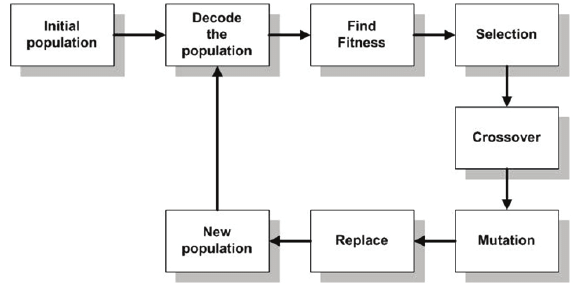
\includegraphics[scale=0.5]{ga_ex.png}
\flushleft
\subsection{Kilka wybranych implementacji powyższych operacji(pseudokod)}
\subsubsection{Selekcja}




\subsubsection{Krzyżowanie}
\paragraph{One-point crossover}-Zamiana suffixów dwóch osobników.
\begin{lstlisting}[language=Python ]
v,w - vectors ( paths)
c = randomint(1,l)
if c!=1:
	for i in (c,l):
		swap(vi,wi)
return v,w
\end{lstlisting}
\paragraph{Two-point crossover}Wymiana genów na zadanym przedziale c,d.
\begin{lstlisting}[language=Python]
v,w - vectors ( paths)
c,d = randomint(1,l),randomint(1,l)
if c>d:
	c,d=d,c
if c!=d:
	for i in (c,d-1):
		swap(vi,wi)
return v,w
\end{lstlisting}
\paragraph{Uniform crossover}Zamiana każdego genu z prawdopodobieństwem p.
\begin{lstlisting}[language=Python]
p - probab of swapping an index
v,w - vectors ( paths)
c,d = randomint(1,l),randomint(1,l)
for i in (1,l):
	if p>random.uniform(0,1):
		swap(vi,wi)
return v,w
\end{lstlisting}
\subsubsection{Mutacja}
\paragraph{Swap} Zamiana genów na pozycjach ( losowych i,j).
\begin{lstlisting}[language=Python]
i,j - random cities range(0,n)
return swap(path,i,j)
\end{lstlisting}
Teraz znając przykładowe implementacje operacji w algorytmie genetycznym głównie opierające się na permutacjach, możemy zacząć rozważania. Możemy postawić, że naszym celem jest znalezienie jak najbardziej optymalnego rozwiązania w jak najkrótszym czasie. Problemem stają się lokalne optima, których musimy pokonać odpowiednio dobierając operacje mutacji, krzyżowania oraz selekcji. Rozważmy kilka solucji problemu komiwojażera wykorzystując optymalny algorytm genetyczny.
\section{Różne strategie selekcji}
Jedną z operacji w algorytmie genetycznym jest selekcja. Służy do wybrania osobników, które następnie chcemy skrzyżować. Przy doborze rodziców musimy uważać, żeby nasze wybory nie doprowadziły do zamknięcia się na jeden genotyp
\subsection{Tournament Selection}
Bardzo popularną metodą jest selekcja turniejowa. Z większej populacji wybieramy x przedstawicieli losowo, wielkość x nazywamy rozmiarem turnieju. Binary Tournament zatem, to selekcja, w której do konkurencji wybieramy tylko 2 chromosomy. Następnie z wyodrębnionego zbioru wybieramy najlepszego. Takie podejście pozwala zachować różnorodność.\\
\centering
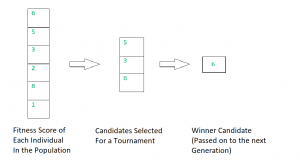
\includegraphics[scale=1.0]{ts.png}\\
\begin{lstlisting}[language=Python]
P - population
t- tounament size >0
best = random.choice(P)
for i from 2 to t:
	next = random.choice(P)
	if fitness(next)>fitness(Best)
		best=next
return best
\end{lstlisting}
\flushleft
\subsection{Proportional Roulette Wheel Selection}
Osobniki są wybierane z prawdopodobieństwem bezpośrednio proporcjonalnym do ich jakości (f -fitness value). Odpowiada to nieco kole ruletki.Koło możemy podzielić na segmenty odpowiadające proporcjom rodziców. Prawdopodobieństwo takie możemy wyznaczyć korzystając z wzoru $p_i=\frac{f_i}{\sum_{j=1}^nf_i}$. Główną zaletą jest to, że żaden z elementów populacji nie zostaje przekreślony. Ma też niestety swoje wady to znaczy, że jeśli populacja początkowa zawiera załóżmy, 2-3 silne genotypy, ale nie idealne, a pozostali członkowie populacji są bardzo słabi - zamknie się na tych dwóch najlepszych ( prawdopodobnie). Z drugiej strony słabe rozwiązania są szybko eliminowane. Jednak jeśli rozważamy problem minimalizacji to jest nieco uciążliwe rozwiązanie, bo musimy zaimplementować funkcje konwertującą funkcje minimalizującą do maksymalizującej. Wprowadza zatem lekkie zamieszanie.\\
\begin{center}
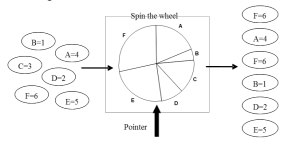
\includegraphics[scale=.8]{pwr.png}
\end{center} 
\begin{lstlisting}[language=Python]
do once per generation
	global p = [ind_1,...,ind_ps]
	global f = [fitness(pi) for pi in p]
	if f is all 0.0s:
		convert f to all 1.0s
	for i from 2 to l:
		fi = fi+ f_{i-1}
perform each time
	n = random(0,fl)
	for i from 2 to l:
		if  f_{i-1}<n<=fi:
			return pi
   return p1
\end{lstlisting}
\subsection{Rank-based Roulette Wheel Selection}
Prawdopodobieństwo wybrania chromosomu jest tutaj zależna od fitness value oraz jest relatywna do całej populacji. Najpierw osobnicy zostają posortowani zgodnie z ich jakością, a następnie wyliczane jest prawdopodobieństwo  na podstawie ich rankingu ,a nie bezpośrednim fitness. Potrzebujemy funkcji mapującej indeksy na posortowanej liście do listy jej prawdopodobieństw selekcji. Funkcja ta może, ale nie musi być liniowa. Bias może być regulowany przy użyciu nacisku wyboru SP dla liniowej np 2>SP>1. Pozycja zatem może być skalowana zgodnie z formułą:\\
$$Rank(Pos)=2-SP + (2.(SP-1).\frac{Pos-1}{n-1})$$ 
Można uniknąć skalowania, ale to może stać się bardziej kosztowne obliczeniowo z powodu sortowania. Takie podejście pozwala zablokować sytuację powodującą utknięcie w najlepszych chromosomach początkowych. Różnica pomiędzy kołami ruletki dla odpowiednio proporcjonalnej i rank-based selekcji.
\begin{center}
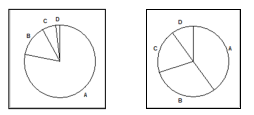
\includegraphics[scale=1.0]{rb.png}\\
Porównanie selekcji:
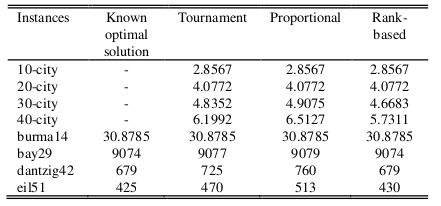
\includegraphics[scale=.7]{cs.png}
\end{center}
\section{Algorytm genetyczny bazujący na entropii}
\subsection{Opis}
Aby poradzić sobie z problemem lokalnego optimum Yasuhiro TSUJIMURA and Mitsuo GEN zaprezentowali rozwiązanie bazujące na entropii. Wykorzystali operację cycle crossover, swap mutation oraz selekcję - roulette wheel selection. Jak wiemy zwiększenie się ilości podobnych chromosomów w populacji może doprowadzić do utknięcia w lokalnym optimum. W EBGA mierzymy różnorodność chromosomów w każdej nowej generacji i ulepszamy populacje o małej różnorodności. Jak wyznaczyć zatem różnorodność? \\
\centering
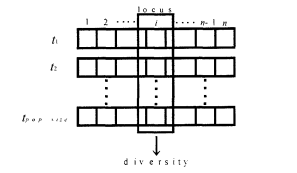
\includegraphics[scale=.7]{locus.png}\\
\flushleft
w tak ustawionych chromosomach przechodzimy po każdej kolumnie i sprawdzamy w niej różnorodność. Locus diversity $H_i$ i-tego locus możemy wyznaczyć ze wzoru:
$$H_i= \sum_{c \in C}pr_{ic}ln(pr_{ic})$$, gdzie
$pr_{ic}=\frac{na_{ic}}{population_{size}}$\\
C - zbiór miast\\
$ na_{ic}$ -ilość wystąpień miasta c na(index kolumny) locus i 
$ H_i $ osiąga maksymalną wartość $ln(population_{size})$, gdy każde miasto z C występuje jednolicie, a 0 gdy jedno z miast występuje znacznie częściej niż pozostałe. $H_i$ musimy oceniać na podstawie jakiejś stałej ( próg(ang. threshold)) w tym przypadku $ln2$.Jeśli próg jest większy lub równy $H_i$ to mamy niską różnorodność. Każde umiejscowienie porównujemy z progiem i jeśli jest większe od 
$\frac{n}{a}$ to zwięksamy podzielność. Parametr a to po prostu integer z przedziału [2,5]. Jak zwiększyć różnorodność? Korzystamy z procedury Med - Pop to znaczy, wybieramy $m=random(\frac{pop_{size}}{a},pop_{size}-1)$ chromosomów z populacji. W każdym wybranym chromosomie wymieniamy geny wzdłuż loca z innym mającym mniejszą różnorodność na locus niż próg.

\subsection{Podsumowanie}
\begin{enumerate}
\item Wygeneruj $pop_{size}$ chromosomów losowo.
\item Ewaluacja wyznacz jakość każdego chromosomu ( fitness) i oceń, który jest najlepszy $eval(t_k) = \frac{1}{\sum_{i=1}^{n}d(c_i,c_{i+1})+d(c_n,c_1)}$
\item Krzyżowanie CX cycle crossover na wybranych chromosomach z prawdopodobieństwem pr
\item Mutacja zamiana miast z prawdopodobieństwem pm
\item selekcja wybierz $pop_{size}$ chromosomów korzystając z roulette wheel selection.
\item Ulepsz różnorodność populacji korzystając z procedury med-pop.
\end{enumerate}
\centering
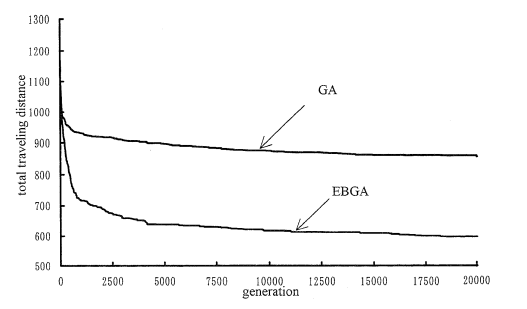
\includegraphics[scale=0.5]{ebga_ga.png}\\
\flushleft
Jak widać EBGA znajduje dużo lepsze rozwiązania niż GA.
\section{Algorytm genetyczny metodą losowych kluczy dla GTSP}
Tak jak już wspomnieliśmy GTSP to zgeneralizowany wariant powszechnie znanego TSP. Różnica polega na tym, że nie każde z miast musi zostać odwiedzone. Mianowicie zbiór miast C jest dzielony na m zbiorów rozłącznych tak, by ich suma była równa C, tzn każde miasto musi należeć do jakiegoś zbioru $C_i$. Tsp jest zatem specjalnym przypadkiem GTSP takim, że C jest podzielone na |C| podzbiorów. W tym przypadku skorzystamy z operacji reprodukcji, czyli skopiowaniu najlepszych elementów z populacji do nowej generacji. W tym problemie skorzystamy również z random keys w celu kodowania rozwiązań. Użycie ich jest możliwe, gdy nasz problem może opierać się na permutacjach integerów i , w których one- lub two- point crossover stwarza problemy. Przeanalizujmy metodę random- key na przykładzie. 
Załóżmy, że mamy ścieżkę 4 2 1 5 3 , nadajemy kolejnym elementom losową wartość ( random key) na przedziale (0,1) i teraz do naszych kluczy przyporządkujemy wartości ze zbioru {1,...,n} rosnąco.
to znaczy, że jeśli mamy 0.1 0.42 0.3 0.9 0.7 to nasz ciąg zostanie zakodowany na 1 3 2 5 4. Wróćmy do naszego zbioru C podzielonego na  załóżmy 3 podzbiory $C_i,C_j,C_k$. Najpierw wykorzystując random keye decydujemy w jakiej kolejności odwiedzimy grupy miast załóżmy, że i -> j -> k. Następnie losujemy klucze dla grup miast i decydujemy o kolejności w tych podgrupach. W tym przypadku 20\% populacji będzie przekazane do nowej generacji, 70\% stworzone przez crossover, a pozostała część zostanie wygenerowana przez imigracje. Przy reprodukcji korzystamy z strategii elitizmu. Pozwala to na zachowanie odpowiednich do mieszania genów.  Do stworzenia potomków używamy uniform crossover. Operacja imigracji co jakiś czas dodajemy po prostu generujemy nowe losowe rozwiązania, które dołączamy do nowej populacji. Ulepszenie każde nowe rozwiązanie uzyskane w GA staramy się poprawić swapując losowe miasta. Druga operacja to 2-opt próbująca usunąć dwa miejsca i wstawić je w inne miejsca tak, aby uzyskać pojedynczy tour o niższym koście. Swap pozwala zamienić miasta z innych komponentów $C_i$. Populacja zarządzamy w taki sposób, aby nie dodawać duplikatów, duplikaty to takie chromosomy, których ulepszenia są takie same. Zalety takiej implementacji to prostota implementacji, jest łatwa do przekształcenia dla innych problemów np MTP lub TCP. Schemat byłby niemal identyczy.
\section{Algorytm genetyczny z mixed region search dla ATSP}
W asymetrycznym TSP mamy do czynienia z różnymi dystansami z miasta A do B, a miasta B do A. Większość algorytmów stworzonych dla STSP mogą zostać zmodyfikowane do ATSP. Mamy n miast do zwiedzenia. Problem ATSP może być sformułowany w następujący sposób:
$$ min \sum_{i=1}{n}\sum_{j=1}{n}x_{ij}c_{ij}$$, gdzie x $\in$  =1 gdy, jest jest takie bezpośrednie połączenie pomiędzy miastami i oraz j na naszej trasie lub 0, gdy nie jest. Liczba rozwiązań niewykonalnych dla ATSP z dwiema podtrasami f(n,2) może być znaleziony w taki sposób: \\
$$f(n,2)=\sum_{i=2}^{floor(0.5n)}$$, gdzie h to ilość niewykonalnych solucji, gdzie i to ilość nodów w jednej podtrasie, a druga ma  n-i nodów. W tym algorytmie bardziej przykuwamy uwagę do operacji krzyżowania. Nasze wyniki mają być później przepuszczone przez patching algorytm Karpa.PMX i TBX czyli partially matched crossover oraz tie break crossover. TBX, którego będziemy jest lekko zmodyfikowany względem standardowego. Najpierw dzielimy naszą trasę tak jak w 2-point crossover. Następnie wybieramy losową ilość elemntów do wymiany i produkujemy nie prawidłową trasę ( z powtórzeniami miast). Kolejno losujemy losowe uniformy na przedziale 0,1 tak jak w random-key values dla miast powtarzających się tzn 1919 generuje 0.1 0.2 0.3 0.4 ciąg  ( losujemy dwa takie wektory) i dodajemy do naszych ścieżek w powtórzeniami Teraz wartości mniejsze przechodzą do mniejszej z zamienionych, a wartości większe do większych ( względem tych, które na początku podmieniliśmy). Dla Uproszczenia przykład:\\
Wybrane jednostki:\\
$$ (1 2 3 | 4 5 6 7 | 8 9)$$
$$ (4 5 2 | 1 8 7 6 | 9 3)$$
Mieszamy, tworzymy szlaki z powtórzeniami:\\
$$ (1 2 3 | 1 8 6 7 | 8 9)$$
$$ (4 5 2 | 4 5 7 6 | 9 3)$$
Losujemy uniformy:\\
$$ 0.3 0.6 0.7 0.3 $$
$$ 0.3 0.5 0.6 0.2 $$
Dodajemy:\\
$$ (1.3 2 3 | 1.6 8.7 6 7 | 8.3 9)$$
$$ (4.3 5.5 2 | 4.6 5.2 7 6 | 9 3)$$
Pozbywamy się powtórzeń:\\
$$ (1 2 3 | 4 8 7 6 | 5 9)$$
$$ (1 8 2 | 4 5 6 7 | 9 3)$$
Do reprodukcji wykorzystujemy stochastyczne próbkowanie z zamianą. ( relatywny ranking względem fitness). W celu mutacji korzystamy z three way -swapping. Korzystamy z niej, gdy nie ma żadnych zmian w wartościach funkcji fitness. W każdej iteracji wybieramy grupę elitarną 60\% . Nasze rozwiązanie poza grupami elitarnymi utrzymuje dobre rozwiązania - nie wpada w lokalne optima. Z każdej grupy 60/30/10 wybieramy przedstawicieli i mixujemy. Raz na jakiś czas do naprawienia rozwiązań, bo w naszym algorytmie generujemy błędne używamy patching algorytm. Graf porównujący:
\begin{center}
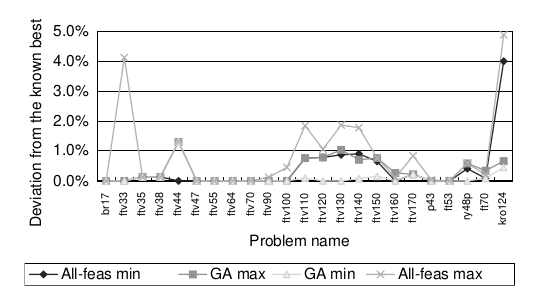
\includegraphics[scale=.7]{mrs.png}
\end{center}
Wyniki wskazują na to, że genetyczny algorytm może być wykorzystany w problemie asymetrycznym TSP i osiągnąć bardzo dobre wyniki.
\section{Algorytm genetyczny dla MOTSP( multi- objective)[ FRAMEWORK PROPOSITION]}
Motsp polega na tym, ze skupiamy się na zminimalizowaniu lub zmaksymalizowaniu wielu funkcji np cost, distance. Jakość solucji jest ewaluowana na podstawie optymalności Pareto. Solucje takie mogą być dominujące lub nie. Zbiór dominujący, inaczej optymalność Pareo to zbiór rozwiązań, które przekłamują w przestrzeni wykonalno- decyzyjnej. Model matematyczny MOTSP:\\
\begin{center}
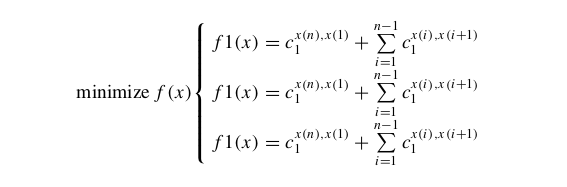
\includegraphics[scale=0.7]{mmotsp.png}
\end{center},gdzie n to ilość miast, $c_j$ to koszt do j, a  to cykliczna permutacja n miast. Euclidean distance jest wykorzystywany do wygenerowania kosztu oraz macierzy dystansów. Dla dwóch wymiarów mamy formułę:\\
$$ECD = \sqrt[2]{(x_2-x_1)^2 + (y_2-y_1)^2}$$.
Na podstawie tego wzoru określamy dystans pomiędzy dwoma miastami. A Pareto jest wykorzystywany do wydobycia rozwiązań efektywnych. Algorytm:
\begin{enumerate}
\item Wczytaj dane dla multi- objective instaces( Euclid)
\item Znajdź dystans dla instancji korzystając Z ECD
\item Macierz jest formowana zgodnie z danym miastem.
\item GA dla tak wygenerowanej macierzy.
	\begin{enumerate}
	\item Stwórz losową populację z macierzy.
	\item Określ jakość chromosomów.
	\item Skrzyżuj wybranych rodziców lub zmutuj
	\item Sprawdź jakość rozwiązań nowych. 
	\end{enumerate}
\item Zwróć najlepszą trasę z odpowiednim kosztem i dystansem.
\end{enumerate}
\begin{center}
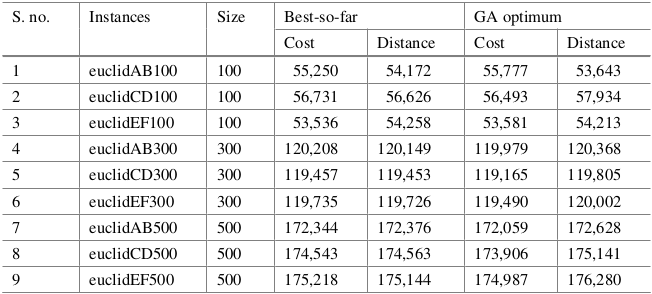
\includegraphics[scale=.5]{rank.png}
\end{center}
GA zoptymalizowało  wszystkie pozycje i znajduje minimalne koszty/dystanse. MOTSP daje przybliżone Pareto optymalne solucje dla każdej pozycji w racjonalnym czasie. Dla EuclidCD100 :\\
\begin{center}
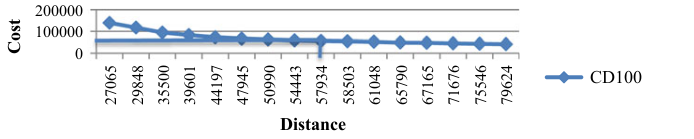
\includegraphics[scale=0.6]{ecd100.png}
\end{center}
Znaczy to tyle, że GA dla problemu MOTSP to bardzo dobry wybór.
\section{Rozwiązanie problemu TSP wykorzystując algorytm genetyczny w rzeczywistej aplikacji}
W tej sekcji zderzymy się z brutalną rzeczywistością i ilością danych jakie musimy przeanalizować. Nasze goals to:\\
\begin{enumerate}
\item Zmniejszyć koszt i czas podróży sprzedawcy.
\item Zwiększyć ilość odwiedzanych na dzień.
\item Priorytetować pewnych klientów.
\item Uwzględnić dni pracy i weekendy oraz nadgodziny.
\end{enumerate}
Jednocześnie chcemy jednak zadbać o \begin{enumerate}
\item odpowiednio się przygotować,
\item ulepszać relacje z klientami,
\item zwiększać pewność siebie sprzedawców,
\item poprawić wydajność firmy ( ogólną),
\item zmniejszyć koszty,
\item zoptymalizować czas pracy.
\end{enumerate}
Dodatkowo musimy uwzględnić rzeczy jak  dni wolne, przerwy śniadaniowe, przystosować czas pracy do godzin porannych, dni preferowane do odwiedzin przez klientów.
W celu rozwiązania problemu musimy skonstruować pewien optymalny model. Zacznijmy od minimalizacji kosztu. 
$$ ovr_cost = distance(R) * km_cost + total_hours(R) * hour_cost$$
gdzie R jest danym rozwiązaniem, dystans sumą sub- tras. Totalny czas możemy wyliczyć z formuły 
$$ total_hours(R)=driving_time(R)+waiting_time(R) + service_time(R)+lunch_time(R)$$ Nasz pesymistyczny przypadek kosztu na godzinę to $worst = hour_cost + speed * km_cost$. Znormalizujmy funkcję
$$norm_cost_per_h(R)= \frac{\frac{overall_cost}{total_hours(R)}}{worst}$$. Przejdźmy do maksymalizacji ogólnej ważności klienta. Ważność klienta będzie najlepiej oceniona jeśli osiągnie max, gdy priorytetowi klienci zostaną odwiedzeni w odpowiednich - porannych godzinach, zatem:\\
$$ importance_{overal}(R)=\sum^H_{d=1}(\sum^N_{i=1}IMP_i * DAYWEIGHT_d * VISIT_{R,i,d})$$, visit mówi o tym ile razy powinien być odwiedzony dany klient. Aby tą funkcję znormalizować musimy znowu sprawdzić extrema.W najgorszym przypadku importance =0, kiedy klient nie został odwiedzony. W najlepszym Każdy zostaje odwiedzony w porannej odpowiedniej porze.
$$importance_{best}= \sum^N_{i=1} IMP_i*DAYWEIGHT_1*FREQMAX_i$$
as
$$ norm_importance(R)= importance_{overall}(R)/ importance_{best}$$
Kolejny czynnik, który chcemy usprawnić to minimalizacja ilości kierunków, które nie były odwiedzane. Mimo wszystko chcemy zwiedzić jak największa ilość klientów w czasie podróży, ale nie naruszając czasu pracy sprzedawcy. $$visits_{max}=\sum^N_iFREQMAX_i$$
$$visited(R) = visits_{max} =\sum^H_{d=1}(\sum^N_{i=1}VISIT_{R,i,d})$$ 
$$ wvisited(R)=visits_{max} - visited(R)$$ Zatem optymalizując nasz problem zbiega do zminimalizowaniu funkcji fintess(R), gdzie 
$$fitness(R)=( a * normCostPerHour(R) +
b * ( 1 - normImportance(R) ) ) *
( c * unvisited(R) + 1 )$$. Nasza reprezentacja wyglądaj ka w poprzednich sekcjach są to ciągi miast 1 2 3 ... Czasem Trasa może mieć kilka dni. Jako operację krzyżowania skorzystamy z omówionego już PMX 
\begin{center}
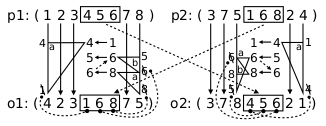
\includegraphics[scale=1.0]{pmx.png}
\end{center}
Z takim podejściem nie musimy się martwić o duplikaty miast. Korzystamy z EM ( Exchange Mutation)
\begin{center}
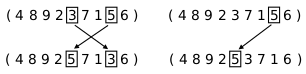
\includegraphics[scale=1.0]{ex.png}
\end{center}
Dla uproszczenia nasze współczynniki a,b,c stawiamy na 1.
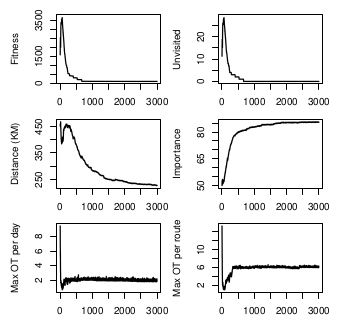
\includegraphics[scale=1.0]{gr1.png}
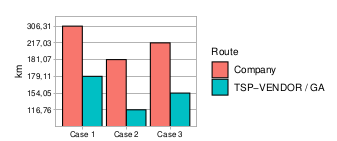
\includegraphics[scale=1.0]{gr2.png}
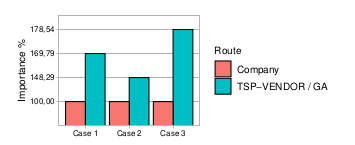
\includegraphics[scale=1.0]{gr3.png}
\section{Podsumowanie}
Często duża wiedza daje duże możliwości, w naszym przypadku tą wiedzą staje się znajomość algorytmów metaheurystycznych. W rzeczywistości często napotykamy na różnego rodzaju problemy. Może się zdarzyć, że nasz problem można przybliżyć do pewnego istniejącego już problemu. Tak jak TSP w powyższym przykładzie, odpowiednie modelowanie i modyfikacje problemu mogą go zgeneralizować lub dopasować się do naszej sytuacji. Algorytm genetyczny jest natomiast jest inteligencją obliczeniową, która pozwala nam z takim problemów ( tutaj NP-trudnych) wybrnąć.

\end{document}